%_____________________________________________________________________________________
%
%       Filename:  chapter1.tex
%
%    Description:  Thesis Template HS Offenburg
%
%
%         Author:  Okba ZOUEGHI, okba.zoueghi@gmail.com
%     Supervisor:  Andreas Walz, Chadlia Jerad
%   Organization:  HS Offenburg, Offenburg, Germany
%
%_____________________________________________________________________________________

\chapter{General Context}

\section*{Introduction}

In this chapter, we see a brief presentation of the host organism and we present the problematic as
well as the objective and the proposed solution.

\section{Presentation of the Host Organism}

The Institute of Reliable Embedded Systems and Communication Electronics (\ac{ivESK})
at the University of Applied Sciences Offenburg was formed to focus on
wired and wireless networks of embedded systems, as well as their interconnection in Cyber-Physical Systems (CPS).
\ac{ivESK} is especially active in designing and implementing of efficient and modular, wired and wireless communications protocols using embedded systems,
for instance, 6LoWPAN, wireless M-Bus, and wired M-Bus. Furthermore, the \ac{ivESK} also designs and implements
integrated security architectures for communication solutions using embedded systems. Actually, Those security architectures
are mostly based on \ac{TLS} and \ac{DTLS}. \ac{ivESK} not only provides communication security, also,
it provides efficient and secure solutions for embedded computing platforms such as Embedded Linux and virtualization.
Last but not least, \ac{ivESK} provides End-to-end security solutions between resource-restricted devices and powerful components.

\section{Problem Description}
During the past 30 years, the main focus in the development of field area networks or, in other words, Industrial networks was on meeting the technical requirements such as real-time constraint and human and machinery safety, resulting in a wide diversity
of systems. These systems were mostly developed as closed environments without interfaces to
outside, partly also because of missing of network solutions. Thus security never played a
prominent role and was not a primary concern in Fieldbus systems \cite{zurawski2014industrial}.

With the introduction of Ethernet in automation, the usage of \ac{TCP}/\ac{IP} became possible, therefore, the same technologies used in LANs
and on the Internet are available at the field level. Thus the possibility of being attacked from outside has become possible which was not the case for the Fieldbus systems.
However, Fieldbus systems still have security issues because they could be attacked from inside \cite{zurawski2014industrial}.

Security measures for IT systems in any organization aim to achieve three basic security goals,
namely, confidentiality, integrity, and authenticity. These measures protect data from unauthorized
entities and unauthorized manipulation and ensure availability. In addition,
another security goal that is often desired is non-repudiation, which binds an entity to its transacted
commitments.

The currently available industrial networks protocols including SafetyNETp, which is the target protocol of this work, do not provide any security measures.
SafetyNETp is vulnerable to attacks as it enables unauthorized access in a relatively straightforward manner given that all the communications are performed with no authentication, no integrity check, and no encryption \cite{zurawski2014industrial}.

The \autoref{vulnerablenetwork} shows how an industrial network is vulnerable to attacks because of the lack of authentication and integrity checks.
This network interconnects a tank, a temperature sensor, and a heater. The temperature sensor sends cyclically the temperature value to the heater. Based on the
received value the heater performs an action on the tank (whether to heat, continue heating, or stop). A problem can be introduced if a malicious third party has gained access to the network,
this third party can modify the messages being sent by the sensor or send fake temperature values to the heater. Therefore the heater's behavior is affected because it does not have any authentication or integrity check mechanism.
\begin{figure}
\centering
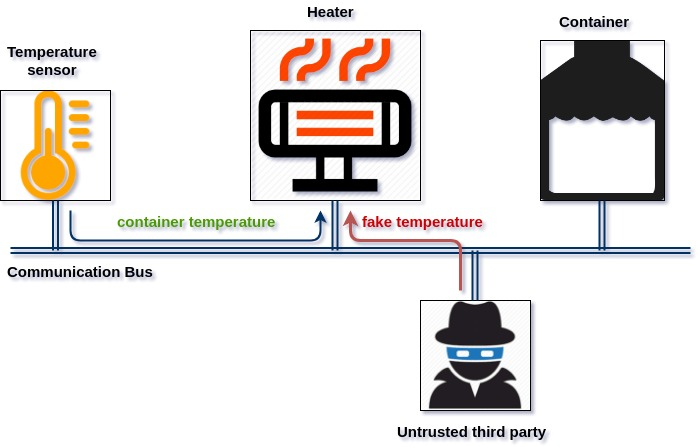
\includegraphics[width=12cm,height=6.5cm]{figures/general_intro/problematic.jpg}
\caption{Lack of authentication exploit}\label{vulnerablenetwork}
\end{figure}

\section{Objective and Proposed Solution}

SafetyNETp is an Industrial Ethernet protocol which provides two communication models, \ac{RTFN} and \ac{RTFL}.
\ac{RTFN} and \ac{RTFL} use different network topologies and operate on different
levels in the \ac{OSI} model. \ac{RTFN} operates on top of both layer two and four, whereas, \ac{RTFL} operates only on top of layer
two. The next chapter will exhibit the difference between these two variants and their respective communication models.
The \autoref{safetynetp_in_osi_model} shows the positioning of \ac{RTFN} and \ac{RTFL} in the \ac{OSI} model.

\begin{figure}[H]
\centering
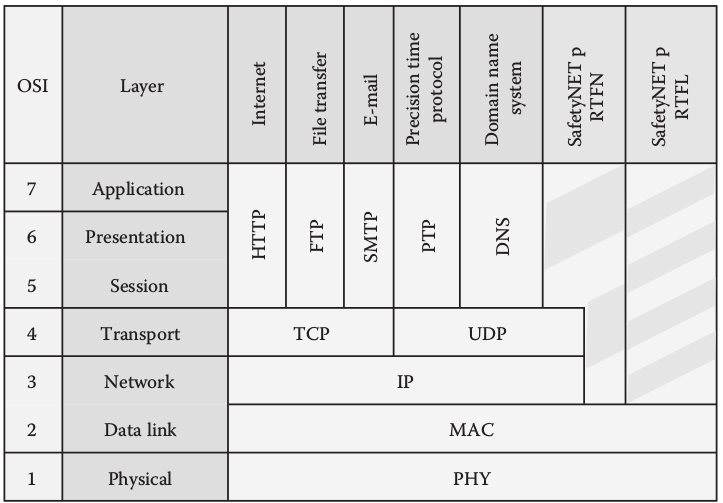
\includegraphics[width=12cm,height=7.5cm]{figures/safetynetp/safetynetp_in_osi_model.png}
\caption[SafetyNETp in the OSI reference model]{SafetyNETp in the \ac{OSI} reference model \cite{pilzSafetyNETpForRealTimeEthernet}}\label{safetynetp_in_osi_model}
\end{figure}
This project aims at securing SafetyNETp RTFN based communication, RTFL being out of the scope of this work; It consists of providing the three basic
security services which are confidentiality, integrity, and authenticity.
Designing a security layer from scratch is a hard and a very error-prone task. That's why we will be interested in the
available solutions which are already tested and assessed by the internet community. \ac{TLS}, \ac{DTLS} and \ac{IPsec} are the most
widely deployed protocols for securing network traffic.
As cited in the general introduction, \ac{TLS} is mostly used for securing
web traffic and e-mail protocols. \ac{TLS} can provide confidentiality, integrity, and authenticity by inserting it between the transport
and the application layers. However, \ac{TLS} provides these security services only for reliable transport protocols such as \ac{TCP}.
The incompatibility of \ac{TLS} with unreliable protocols led to the introduction of \ac{DTLS} which was introduced to provide \ac{TLS}'s security services for unreliable protocols.
Like \ac{TLS} and \ac{DTLS}, \ac{IPsec} provides confidentiality, integrity and authenticity, furthermore, it could be used for securing both
reliable and unreliable protocols.
In the next chapter, we study and we choose the suitable protocol to be used. Our solution consists of
designing and implementing a security layer for SafetyNETp RTFN based on the chosen security protocol.

Our work will involve the following steps :
\renewcommand{\labelitemi}{$\bullet$}
\begin{itemize}
\item Study SafetyNETp protocol
\item Study the available security solutions (\ac{TLS}, \ac{DTLS}, \ac{IPsec}) and choose the suitable one for SafetyNETp
\item Find and analyze the existing implementations of the protocol of choice and select the suitable one
\item Design the security layer and its integration into SafetyNETp
\item Implement and integrate the security layer
\item Test the implemented solution
\end{itemize}

\section*{Conclusion}

After setting the general context, we move in the following chapter to
outline the basic concepts needed for our project and to choose the security
protocol to be used
